\section{Conceptual Design}

\subsection{Variations to the Requirement Analysis}

After a second round of intervews with the Stakeholders we have clarified some doubts: \\
\textbf{Car Dealer} is the local physical car shop and as such has it's own employees, that are: Sellers, Mechanics and the Finance Team. By our design, since the business is constantly growing, any new work role can be easily implemented in the database without problems. Once we clarified that Car Dealer is the single local shop we can continue, as agreed, to identify the different local business by their Names. \\
We made some clarification also about the repair service. As of now it exists only to repair the rentable cars. We discussed if the policy could change in the future, in order to allow repairs to customers too, so we agreed on adding a new entity \textbf{External Cars} related to Customers and Repair current entities. 

\subsection{Entity-Relationship Schema}
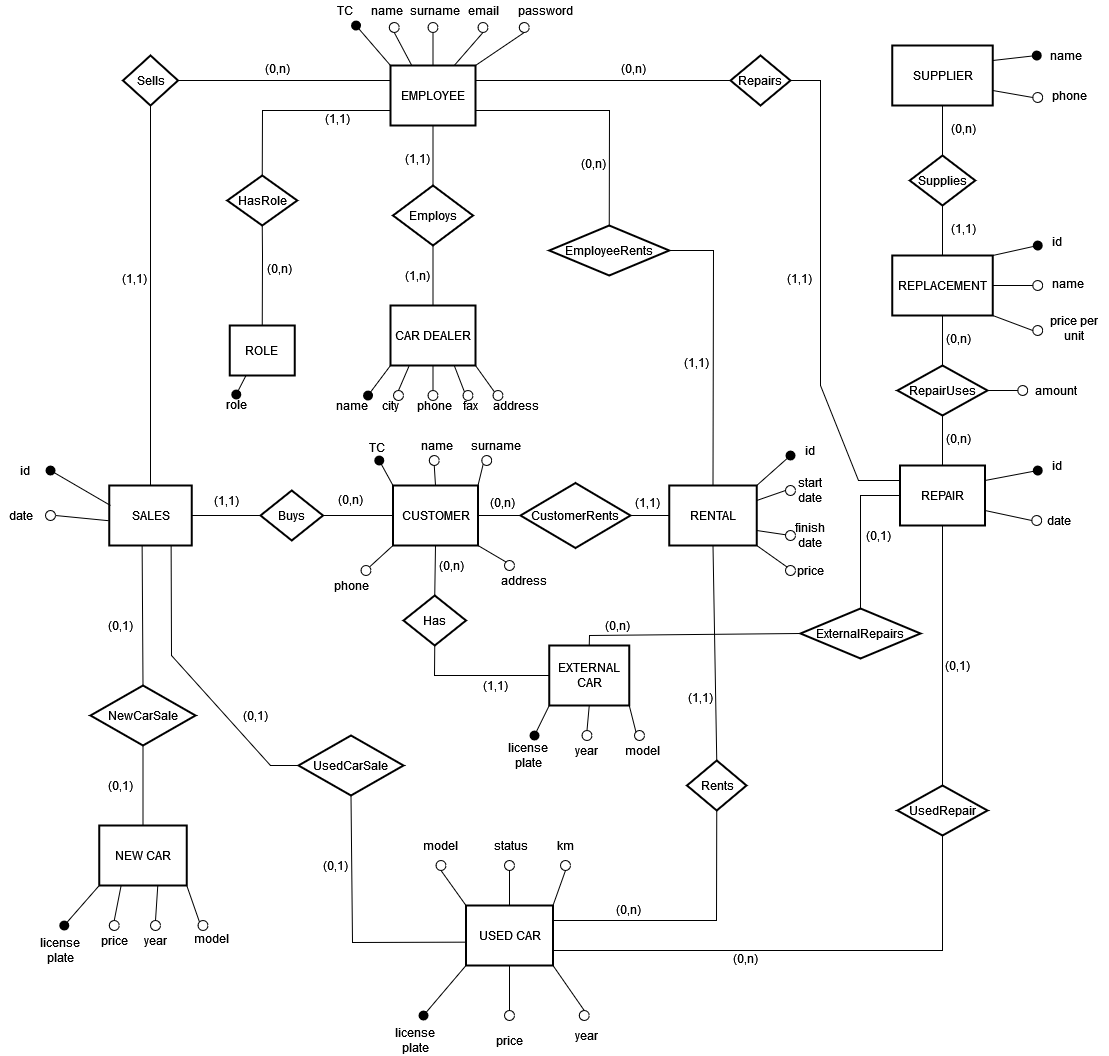
\includegraphics[width=19cm, height=16cm]{ER_final.png}

\subsection{Data Dictionary}

\subsubsection{Entities Table}
\begin{longtable}{|p{.20\columnwidth}|p{.30\columnwidth} |p{.20\columnwidth}|p{.20\columnwidth} |} 
\hline
\textbf{Entity} & \textbf{Description} & \textbf{Attributes} & \textbf{Identifier}  \\\hline


Car Dealer & Business that has the ability to sell or rent cars that may be new or used. Univocally identified by the Car Dealer's name (name of the business). & \begin{itemize}
        \vspace{-1em}
        \item name
        \item address
        \item city
        \item phone
        \item fax
    \end{itemize}
& name\\\hline
 
 Customer & Customer within the car dealer chain, can buy or rent one or more cars. Can also have his/her car repaired. Identified by the Tax Code. & \begin{itemize}
        \vspace{-1em}
        \item TC
        \item name
        \item surname
        \item phone
        \item address
    \end{itemize}
 &  TC \\\hline

 Sales & Contract or invoice between the car dealer and the customer by which a car, new or used, is sold. Each sale is identified by an id. & \begin{itemize}
    \vspace{-1em}
    \item id
    \item date
    \end{itemize}
& id \\\hline

Rental & Contract or invoice between the car dealer and the customer related to the car rental processes of Used Car. Each rental is identified by an id. & \begin{itemize}
        \vspace{-1em}
        \item id
        \item start date
        \item finish date
        \item price
    \end{itemize}
& id\\\hline

New Car & Real world object that can be sold (and only sold) by a car dealer. Each New Car is identified by its license plate & \begin{itemize}
    \vspace{-1em}
    \item license plate
    \item price
    \item year
    \item model
\end{itemize}
&  license plate\\\hline

Used Car & Real world object that can be sold or rented by a car dealer. They are different from New Cars in the system because they may be rented or not, also they may be under repair and therefore not available. Each used car is identified by its license plate& \begin{itemize}
    \vspace{-1em}
    \item license plate
    \item price
    \item year
    \item status
    \item km
    \item model
\end{itemize}
&  license plate\\\hline

External Car & Real world object that doesn't belong to the car dealer but has been processed in the repair service. Identified by a licence plate. & \begin{itemize}
        \vspace{-1em}
        \item licence plate
		\item year
		\item model
    \end{itemize}
 &  licence plate \\\hline
 
 Repair & Repair service that the car dealer offers for the used cars that belong to the branch and external cars. Identified by an id. & \begin{itemize}
        \vspace{-1em}
        \item id
        \item date
    \end{itemize}
 &  id \\\hline

Replacement & A list of replacing parts needed for the repair service. Identified by an id. & \begin{itemize}
    \vspace{-1em}
    \item id
    \item name
	\item price per unit
    \end{itemize}
& id \\\hline

Supplier & A vendor that supplies required parts to the repair service. Identified by an id. & \begin{itemize}
    \vspace{-1em}
    \item name
    \item phone
\end{itemize}
&  name\\\hline

Role & Information in the system that is responsible for keeping track of different roles of various employees. Identified by role. & \begin{itemize}
    \vspace{-1em}
    \item role
\end{itemize}
&  role\\\hline

Employee & Representative of a real person who works at the car dealer. They are registered to the system with their given attributes. Each employee is identified by her/his Tax Code. & \begin{itemize}
    \vspace{-1em}
    \item TC
    \item name
    \item surname
    \item email
    \item password
\end{itemize}
&  TC\\\hline

\end{longtable}


\subsubsection{Relationships Table}
\begin{longtable}{|p{.20\columnwidth}|p{.20\columnwidth} |p{.30\columnwidth}|p{.25\columnwidth} |} 
\hline
\textbf{Relationship} & \textbf{Description} & \textbf{Component Entities} & \textbf{Attributes} \\\hline

Employs & Associates Car Dealer with his Employees. & \begin{itemize}
		\vspace{-1em}
		\item CarDealer (1,N);
		\item Employee (1,1);
	\end{itemize}
 & \\\hline

Buys & A Customer makes a purchase. & \begin{itemize}
		\vspace{-1em}
		\item Customer (0,N);
		\item Sales (1,1)
	\end{itemize}
 & \\\hline

CustomerRents & A Customer makes a rental. & \begin{itemize}
		\vspace{-1em}
		\item Customer (0,N);
		\item Rental (1,1);
	\end{itemize}
 & \\\hline

NewCarSale & Associates a New Car to the Sales in which it was sold. & \begin{itemize}
		\vspace{-1em}
		\item NewCar (0,1);
		\item Sales (0,1);
	\end{itemize}
 & \\\hline

UsedCarSale & Associates a Used Car to the Sales in which it was sold. & \begin{itemize}
		\vspace{-1em}
		\item UsedCar (0,1);
		\item Sales (0,1);
	\end{itemize}
 & \\\hline

RepairUses & Associates a Repairment with the replacement parts that have been used. & \begin{itemize}
	\vspace{-1em}
	\item Repair (0,N);
	\item Replacement (0,N);
\end{itemize}
& amount \\\hline

Supplies & Associates a replacement part with his supplier. & \begin{itemize}
	\vspace{-1em}
	\item Replacement (1,1);
	\item Supplier (0,N);
\end{itemize}
& \\\hline

Rents & Association between Used Cars and Rental. & \begin{itemize}
	\vspace{-1em}
	\item Used car (0,N);
	\item Rental (1,1);
\end{itemize}
& \\\hline

UsedRepairs & Associates an Old Car to a Repair instance. & \begin{itemize}
	\vspace{-1em}
	\item Used car (0,N);
	\item Repair (0,1);
\end{itemize}
& \\\hline

Has & Customer has an external car. & \begin{itemize}
	\vspace{-1em}
	\item Customer (0,N);
	\item External car (1,1);
\end{itemize}
& \\\hline

ExternalRepairs & Customer wants his/her external car to be repaired. & \begin{itemize}
	\vspace{-1em}
	\item External car (0,N);
	\item Repair (0,1);
\end{itemize}
& \\\hline

EmployeeRents & Associates an Employee to a Rental he/she made. & \begin{itemize}
	\vspace{-1em}
	\item Employee (0,N);
	\item Rental (1,1);
\end{itemize}
& \\\hline

Sells & Employee sells an Used or a New Car. & \begin{itemize}
	\vspace{-1em}
	\item Employee (0,N);
	\item Sales (1,1);
\end{itemize}
& \\\hline

Repairs & Associates an Employee to a Repair he/she performed. & \begin{itemize}
	\vspace{-1em}
	\item Employee (0,N);
	\item Repair (1,1);
\end{itemize}
& \\\hline

HasRole & Associates an Employee to his/her Role in the company. & \begin{itemize}
	\vspace{-1em}
	\item Employee (1,1);
	\item Role (0,N);
\end{itemize}
& \\\hline

\end{longtable}


\subsection{External Constraints}
\begin{itemize}
    \item Phone and fax fields should comply with the E.164 standard (i.e. +1 999 555 0123).
    \item Date-valued fields should comply with ISO 8601 standard (i.e. 2011-12-03T10:15:30+01:00)
    \item Money-valued fields must be non-negative Float expressed in Euro.
    % \item Rental prices must be non-negative Float expressed in Euro per month.
    \item The Rental must be longer than a month.
    \item Each year field must be an integer greater than 1900 and less than 9999.
    \item E-mail fields should comply with format defined in the RFC 2821 specification.
    \item Password fields must be hashed according to the RFC 2898 specification.
    \item Sellers must not be able to insert, update or delete repairs.
    \item Mechanics must not be able to insert, update nor delete both sales and rentals.
    \item Finance employees must not be able to insert, update or delete sales, rentals or repairs, but they can still read their values.
    \item Mechanics should be able to manage repairs, in particular adding replacements when needed.
    \item The amount of a given replacement in a single repair must be a positive integer.
    \item For each Sale instance either the NewCarSale relationship or the UsedCarSale one must be present.
    \item For each Repair instance either the ExternalRepairs relationship or the UsedRepairs one must be present.
\end{itemize}

\subsection{Functional Requirements Satisfaction Check}
\begin{itemize}
\item \textbf{Since it is a chain of car dealers, not a single car dealer, manage the different dealers located in different places.}\\\\
	\,
	Car Dealer has more than one branch. All branches’ informations are stored in CAR DEALER entity with their instances as name, city, phone, tax, address.
	\item \textbf{For each car dealer store their sale information.}\\\\
	\,
	The New Car and Used Car sales data is stored in SALES entity, CAR DEALER employs EMPLOYEE and employees has relationship with SALES entity through Sells relationship.
	\item \textbf{For each car dealer store their rental information.}\\\\
	\,
	The Used Car sale data is stored in RENTAL entity.CAR DEALER employs EMPLOYEE and employees has relationship with RENTAL entity through EmployeeRents relationship.
	\item \textbf{Each car dealer's employee have the access to the progress of the activity, in particular can view sales, rentals and repairs regarding cars.}\\\\
	\,
	Employees can access sales, rentals and repairs data with proper priviledges. Each car dealer branch is able to access related branch data in these categories.

	\item \textbf{Manage customer information such as name, surname, address, phone, through their purchases or rental in the car dealer.}\\\\
	\,
	Customers are recorded in the system with their tax code, name, surname, phone and address. They have relationship with cars for sale (Sales entity) through Buy and cars for rental (Rental entity) through CustomerRents. They may have their own cars which are called external cars and have relationship by Has. Car Dealer’s employee can access the customer data.
	\item \textbf{Allow the workers to check how many repairments an used car received.}\\\\
	\,
	Workers data is stored in Employee entity and employees are able to access Repair data which has relationship with Used car by UsedRepair. Employee can see date and id of repair data, thus employee can check how many times the used car has been repaired. 
	\item \textbf{For each repair, keep track of the replacements used in quantity and their price.}\\\\
	\,
	Repair data stored in REPAIR entity with its date and id.
	\item \textbf{Store information of all the suppliers, even if they have never sold a part yet.}\\\\
	\,
    Supplier data is stored in SUPPLIER entity with its name, phone. Even if they never sold any part yet.

    \item \textbf{Each car dealer needs to have a catalog that provides the list of used cars and new cars. }\\\\
    \,
    USED CARS and NEW CARS are accessible through SALES and RENTAL entities by the EMPLOYEE which is employed by CAR DEALER.
    \item \textbf{Check that there is one car dealer associated to each sale / rental. }\\\\
    \,
    CAR DEALER employes EMPLOYEE who sells NEW CARS or USED CARS. EMPLOYEE has the relationship with NEW CARS and USED CARS through SALES entity, also EMPLOYEE has the relationship with USED CARS through RENTAL entity.
    \item \textbf{Check that there is one customer associated to each sale / rental. }\\\\
    \,
     CUSTOMER has the relationship with SALES entity through Buys, also with RENTAL through CustomerRents.
    \item \textbf{Check that there is one new car / used car associated to each sale. }\\\\
    \,
    SALES entity has the relationship with NEW CARS through NewCarSale and with USED CAR through UsedCarSale.
    \item \textbf{Check that there is one used car associated to each rental. }\\\\
    \,
    RENTAL entity has the relationship with USED CAR through Rents.
    \item \textbf{Check that there is one car dealer associated to each repair. }\\\\
    \,
    CAR DEALER employees EMPLOYEE who has the connection with REPAIR entity through Repairs. 
    \item \textbf{Check that there is one supplier associated to each replacement.} \\\\
    \,
    SUPPLIER is connected to REPLACEMENT through the Supplies relationship.
\end{itemize}